% Intended LaTeX compiler: xelatex
\documentclass[a4paper, 12pt]{article}
\usepackage{graphicx}
\usepackage{longtable}
\usepackage{wrapfig}
\usepackage{rotating}
\usepackage[normalem]{ulem}
\usepackage{amsmath}
\usepackage{amssymb}
\usepackage{capt-of}
\usepackage{hyperref}
\usepackage[danish]{babel}
\usepackage{mathtools}
\usepackage[margin=3.0cm]{geometry}
\hypersetup{colorlinks, linkcolor=black, urlcolor=blue}
\setlength{\parindent}{0em}
\parskip 1.5ex
\author{Jacob Debel}
\date{Fysik C \& B}
\title{Lys og bølger\\\medskip
\large Transformation - Simple opgaver}
\hypersetup{
 pdfauthor={Jacob Debel},
 pdftitle={Lys og bølger},
 pdfkeywords={},
 pdfsubject={},
 pdfcreator={Emacs 29.4 (Org mode 9.6.15)}, 
 pdflang={Danish}}
\begin{document}

\maketitle


\section*{Opgave 1}
\label{sec:orgf9bd3b4}
\begin{center}
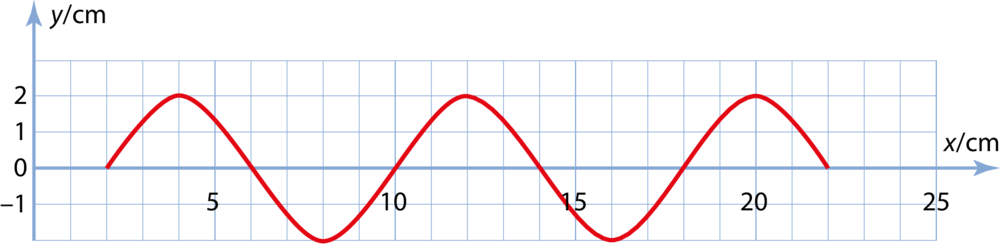
\includegraphics[width=.9\linewidth]{./img/boelge_opgave.png}
\end{center}

\begin{itemize}
\item Bestem ud fra figuren bølgelængde og amplitude for bølgen.
\end{itemize}

\section*{Opgave 2}
\label{sec:orgeb84499}

Lyset fra en helium-neon-laser har en bølgelængde på 632.8 nm.

\begin{itemize}
\item En e-coli-bakterie er typisk 2 \(\mu m\) lang. Hvor mange bølgelængder af laserens lys svarer det til?

\item Et atom har typisk en diameter på 200 pm. Hvor mange atomer kan der ligge ved siden af hinanden på 632.8 nm?
\end{itemize}

\section*{Opgave 3}
\label{sec:orgd12311f}

\begin{itemize}
\item Beregn bølgelængden af lys med frekvensen \(11.3 \cdot 10^{14}\) Hz.
\end{itemize}

\section*{Opgave 4}
\label{sec:orgd8fae74}

En lysstråle sendes med indfaldsvinklen \(i=32^{\circ}\) fra luft ind i et stykke rudeglas.

\begin{itemize}
\item Beregn brydningsvinklen \(b\) i glasset.
\end{itemize}

\section*{Opgave 5}
\label{sec:org1f820df}

En lysstråle sendes med en indfaldsvinkel på \(74,9^{\circ}\) ned gennem en væskeoverflade.

Brydningsvinklen er \(45.3^{\circ}\).

\begin{itemize}
\item Beregn væskens brydningsindeks.
\end{itemize}

\section*{Opgave 6}
\label{sec:org991d7a0}

Lys fra et udladningsrør med hydrogen sendes gennem et optisk gitter med 560 spalter pr. mm.

\begin{itemize}
\item Beregn afbøjningsvinklen \(\phi_1\) til den røde linje (\(\lambda = 656\) nm) i 1. orden.
\end{itemize}

\section*{Opgave 7}
\label{sec:org58dac61}

Gult lys fra en såkaldt natriumlampe sendes gennem et optisk gitter med 300 spalter pr. mm. Afbøjningsvinklen \(\phi_5\) til 5. orden måles til \(58.6^{\circ}\).

\begin{itemize}
\item Bestem lysets bølgelængde.
\end{itemize}

\section*{Opgave 8}
\label{sec:orgdeea034}

Ved et gittereksperiment sendes lys med bølgelængden 400 nm gennem et gitter. På en skærm 3.4 m fra gitteret måles afstanden mellem centralpletten og lyspletten i 1. orden til 136 mm.

\begin{itemize}
\item Beregn gitterkonstanten i det anvendte gitter.
\end{itemize}

\section*{Opgave 9}
\label{sec:org9cd7292}

En lysstråle har en bølgelængde på 650 nm i vakuum.

\begin{enumerate}
\item Hvilken farve har lysstrålen?

\item Hvad er lysstrålens frekvens i vakuum?

\item Hvad er lysets hastighed i en væske, hvis brydningsindeks ved denne bølgelængde er 1.47?

\item Hvad er lysets bølgelængde i væsken?
\end{enumerate}

\section*{Opgave 10}
\label{sec:org713f28a}

En lysstråle sendes fra luft hen mod en glasplade med et brydningsindeks på 1.66. Lysstrålens vinkel i forhold med glasoverfladen er \(47.5^{\circ}\).

\begin{enumerate}
\item Beregn indfaldsvinklen.

\item Beregn brydningsvinklen.
\end{enumerate}

\section*{Opgave 11}
\label{sec:orgd8d064b}

En lysstråle sendes fra luft ind i plexiglas, som vist på figuren. Brydningsindekset for plexiglas kan slås op til at have værdien 1.4914.

\begin{center}
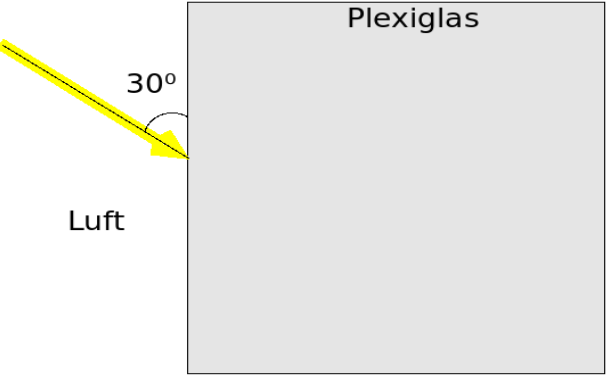
\includegraphics[width=.9\linewidth]{./img/Plexiglas.png}
\end{center}

\begin{enumerate}
\item Indtegn indfaldsvinkel og brydningsvinkel på figuren.

\item Beregn brydningsvinklen.
\end{enumerate}

\section*{Opgave 12}
\label{sec:org343ea4b}

En He-Ne-laser (Helium-Neon-laser) udsender lys med bølgelængden 632.8 nm mod et gitter med ukendt gitterkonstant.
Afbøjningsvinklen til 1. orden er \(30^\circ\).

\begin{enumerate}
\item Bestem gitterkonstanten.

\item Hvor mange linjer pr. mm. har gitteret?
\end{enumerate}

\section*{Opgave 13}
\label{sec:orgab90255}

En kviksølvslampe udsender bl.a. en kraftig blå spektrallinje med en bølgelængde på 435.8 nm. Dette blå lys sendes ind mod et gitter med 660 linjer pr. mm. 

\begin{enumerate}
\item Hvad er den størst mulige afbøjningsorden?

\item Bestem alle de mulige afbøjningsvinkler.
\end{enumerate}

\section*{Facitliste}
\label{sec:orgf3ae3c3}
\textbf{Opgave 1:} \(\lambda=8cm\), amplituden er 2 cm.

\textbf{Opgave 2:} 3 hele bølgelængder (3.16) - 3164 atomer ved siden af hinanden.

\textbf{Opgave 3:} \(\lambda = 265 nm\)

\textbf{Opgave 4:} \(b=21^{\circ}\)

\textbf{Opgave 5:} \(n=1.36\)

\textbf{Opgave 6:} \(\phi_1 =21.6^{\circ}\)

\textbf{Opgave 7:} \(\lambda = 569 \,nm\)

\textbf{Opgave 8:} \(d=0.010 \,mm\) 

\textbf{Opgave 9:} \textbf{1.} Rød, \textbf{2.} \(f=4.62 \cdot 10^{14}\) Hz, \textbf{3.} \(v=2.04 \cdot 10^8 m/s\), \textbf{4.} \(\lambda = 441.5 nm\).

\textbf{Opgave 10:} \textbf{1.} \(i=42.5^{\circ}\), \textbf{2.} \(b=24.02^{\circ}\)

\textbf{Opgave 11:} \textbf{1.} Tegning , \textbf{2.} \(b=35.5^{\circ}\)

\textbf{Opgave 12:} \textbf{1.} d = 1256.6 nm, \textbf{2.} 790 linjer pr. mm.

\textbf{Opgave 13:} \textbf{1.} \(n_{max} = 3\), \textbf{2.} \(\phi_1 = 16.7^{\circ}\), \(\phi_2 = 35.1^{\circ}\), \(\phi_3 = 59.6^{\circ}\)
\end{document}
